\documentclass[11pt,a4paper]{article}
\usepackage[margin=2.5cm]{geometry}
\usepackage[utf8]{inputenc}
\usepackage[T1]{fontenc}
\usepackage{hyperref}
\renewcommand{\familydefault}{\sfdefault}
\usepackage{helvet}
\pagestyle{empty}
%\usepackage[kerning=true]{microtype}
\usepackage{parskip}
\usepackage{sansmath}
\usepackage[font={small, bf}]{caption}
\usepackage[font={small}]{subcaption}
\usepackage{graphicx}
\usepackage{multicol}
\setlength{\abovecaptionskip}{0pt}
\setlength{\floatsep}{10pt}
\setlength{\textfloatsep}{0pt}
\setlength{\intextsep}{0pt}
\setlength{\belowcaptionskip}{0pt}
\setlength{\parindent}{0ex}
\setlength{\parskip}{0pt}
% Feel free to use additional packages for glosses, figures, whatnot.

% The next bit is for reserving sufficient space for authors,
% affiliations, and e-mail address.  No need to change for initial
% anonymous version.  For the final version, replace the
% \toggletrue{anonymous} with \togglefalse{anonymous} to de-anonymize.
\usepackage{etoolbox}
\newtoggle{anonymous}
\togglefalse{anonymous}

\renewcommand{\title}[1]{\textbf{#1}\\}
\newcommand{\authors}[1]{\iftoggle{anonymous}{\phantom{#1}}{#1}\\}
\newcommand{\email}[1]{\iftoggle{anonymous}{\phantom{#1}}{#1}}

\begin{document}

% First page:

% Insert title, authors, affiliations, and e-mail address in the next three lines:
\noindent\title{TODO title goes here}
\authors{Veronica Boyce (Stanford University, vboyce@stanford.edu), Roger P. Levy (MIT)} 
\newline
%


Much linguistic input is ambiguous in isolation, at least as it is incrementally encountered and processed. In particular, various syntactic structures exist that are ambiguous between multiple different attachment structures part way through the input.
Luckily, language we encounter is intended to be informative and communicative, so there are contextual correlations between features of the language itself, the prior linguistic context, and the visual context that can help inform what parse is expected. 

A general question is how rapidly different types of contextual information are used and what tasks can detect them. In the present work, we use the Maze task (CITATIONS) to look at online processing times delays at disambiguation points to explore the role of linguistic and visual context in biasing attachment preferences. Both experiments use the NP versus VP attachment ambiguity. 

\medskip
\noindent\textbf{Experiment 1: Linguistic context} We used the materials from Altmann \& Steedman (1988) study N to see if the Maze task would reveal influences on attachment preferences based on the described context (see reverse for sample item). In clause by clause SPR, A \& S had found an interaction where NP modifiers were preferred in the 2-referent condition (when needed to disambiguate *which* map), but VP modifiers where preferred in the 1-referent condition. We recruited 100 participants to read TODO number of items in an A-Maze paradigm. For the 88 participants who had greater than 80\% selection accuracy, we found an expected interaction effect of 84 ms [95\% CI 17-148ms] on the disambiguating words. Participants read words faster in the 2-referent NP and 1-referent VP conditions, indicating that preferred parse was influenced by whether the context supported the presence of a restrictive modifier.  This confirmed that the Maze task can localize syntactic parsing differences that interact with linguistic context. 

\medskip
\noindent\textbf{Experiment 2: Visual context} Visually presented context appears to affect online sentence parsing in visual world tasks (the 1995 paper, kpath). When there is only one object that matches a noun, the following PP is initially interpreted as a VP-attached goal location (judging by eye movements). When there are two objects, the PP seems to be immediately interpreted as a restrictive NP-attached modifier. This leads to strong reanalysis penalties when an another PP (the true goal) occurs, but only in 1-referent conditions. We are not aware of any incremental reading paradigms being used with co-occurring visual context. We set up a Maze task where a context image was displayed for N seconds and then stayed visible as the maze selections appeared below (Figure TODO). We used some items based on TODO weighall or whatever, and we recruited 200 participants who each saw 4 critical items (1/condition) mixed with 4 fillers. Distractor words were generated using the A-Maze paradigm. 

We found expected RT effects from linguistic conditions (increased RT at TODO), but no effects from the visual context or visual context interaction. 

\medskip
\noindent\textbf{Discussion:} Online ambiguity resolution is important, but many forms of context can constrain the interpretation of utterances. However, it is unclear under what conditions different types of information affect linguistic processing how quickly, or what experimental paradigms are sufficient to detect them. Here, we demonstrate that context presented linguistically does affect Maze RTs, but that co-presented visual context does not, unlike in visual world paradigms. This different could be due to high cognitive load from Maze and lack of task reason to closely inspect the image, or the two tasks could be querying different stages in linguistic processing and interpretation. 

TODO future work 
TODO are there ERP studies on this? 
TODO can I assume people know the Maze task at this point? 
TODO possibly link to where expts can be tried out? 

\newpage

\begin{minipage}{\textwidth}
\begin{small}
Experiment 1 example stimuli:\\
\textit{(context)} A historian was working in the British Museum holding a magnifying glass. He'd sat down to study  a map. \\
\textit{(1 or 2 referent)} On his desk there was \textbf{a map} which had an appalling tear and \textbf{a  {[manuscript | map]}} which seemed in perfect condition. \\
\textit{(NP or VP attachment)} The historian had to study \textbf{the map with the {[appalling  tear | magnifying glass]}} so as to value it.
\end{small} 
\end{minipage}










\begin{minipage}{.5\textwidth}
	\captionof{figure}{Results}
	{	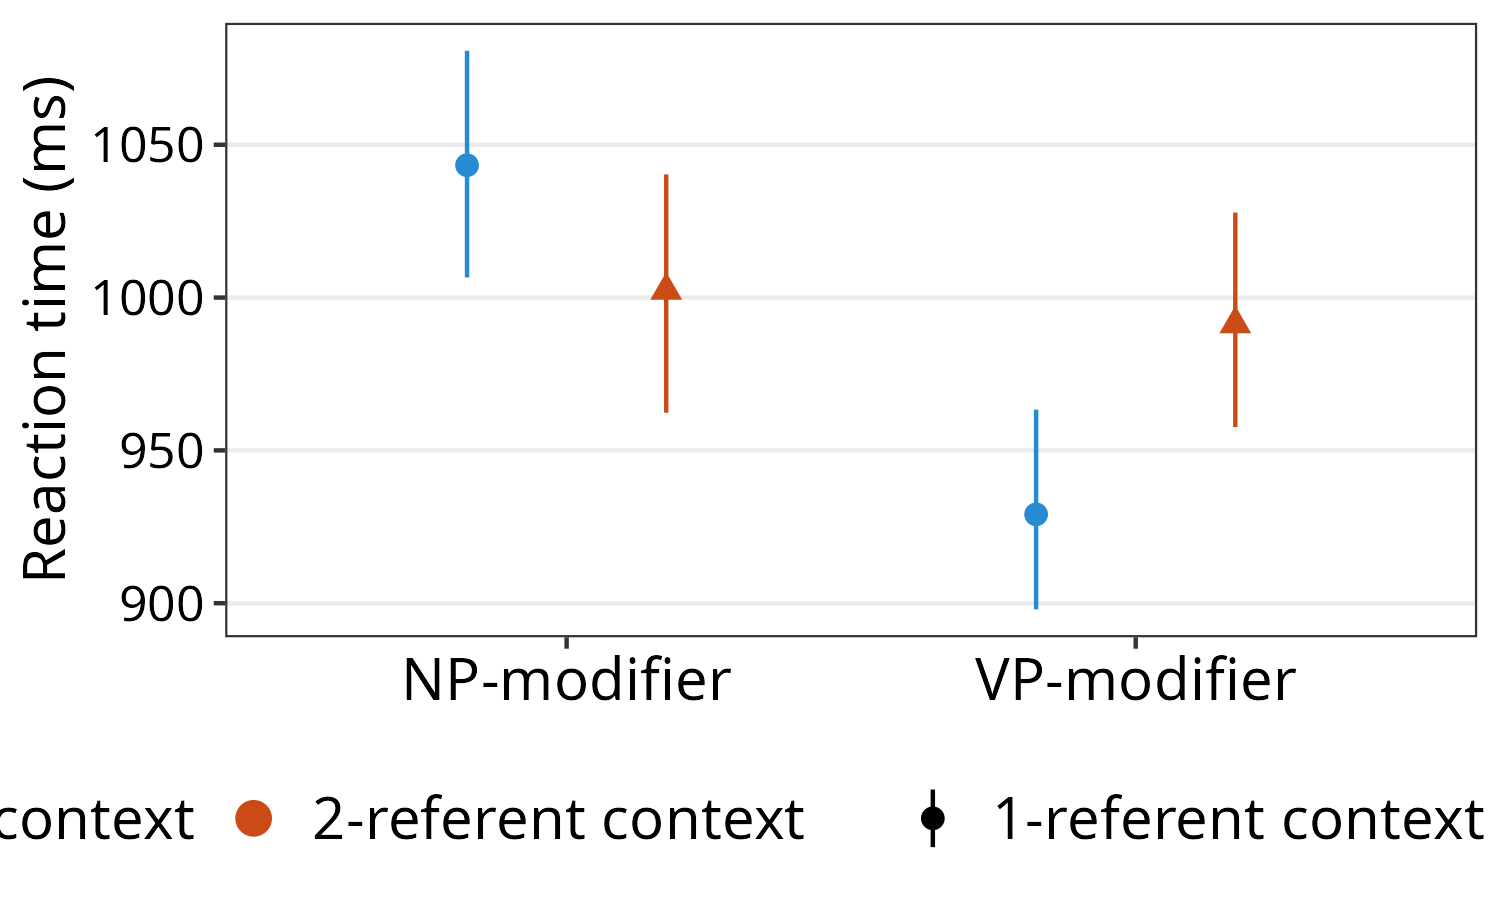
\includegraphics[width=\textwidth]{nrsa.png}} 
	\begin{small}
	CAPTION HERE
		
	\end{small}
	
\end{minipage}
~~~
\begin{minipage}{.5\textwidth}	
	\begin{tabular}{l}
		TODO results table here\\
	\end{tabular}
\end{minipage}

\begin{minipage}{\textwidth}
	Experiment 2 materials: 2 sentences x 2 images
	
	
\end{minipage}
	
	
	\begin{minipage}{.5\textwidth}
		\captionof{figure}{Results}
		{	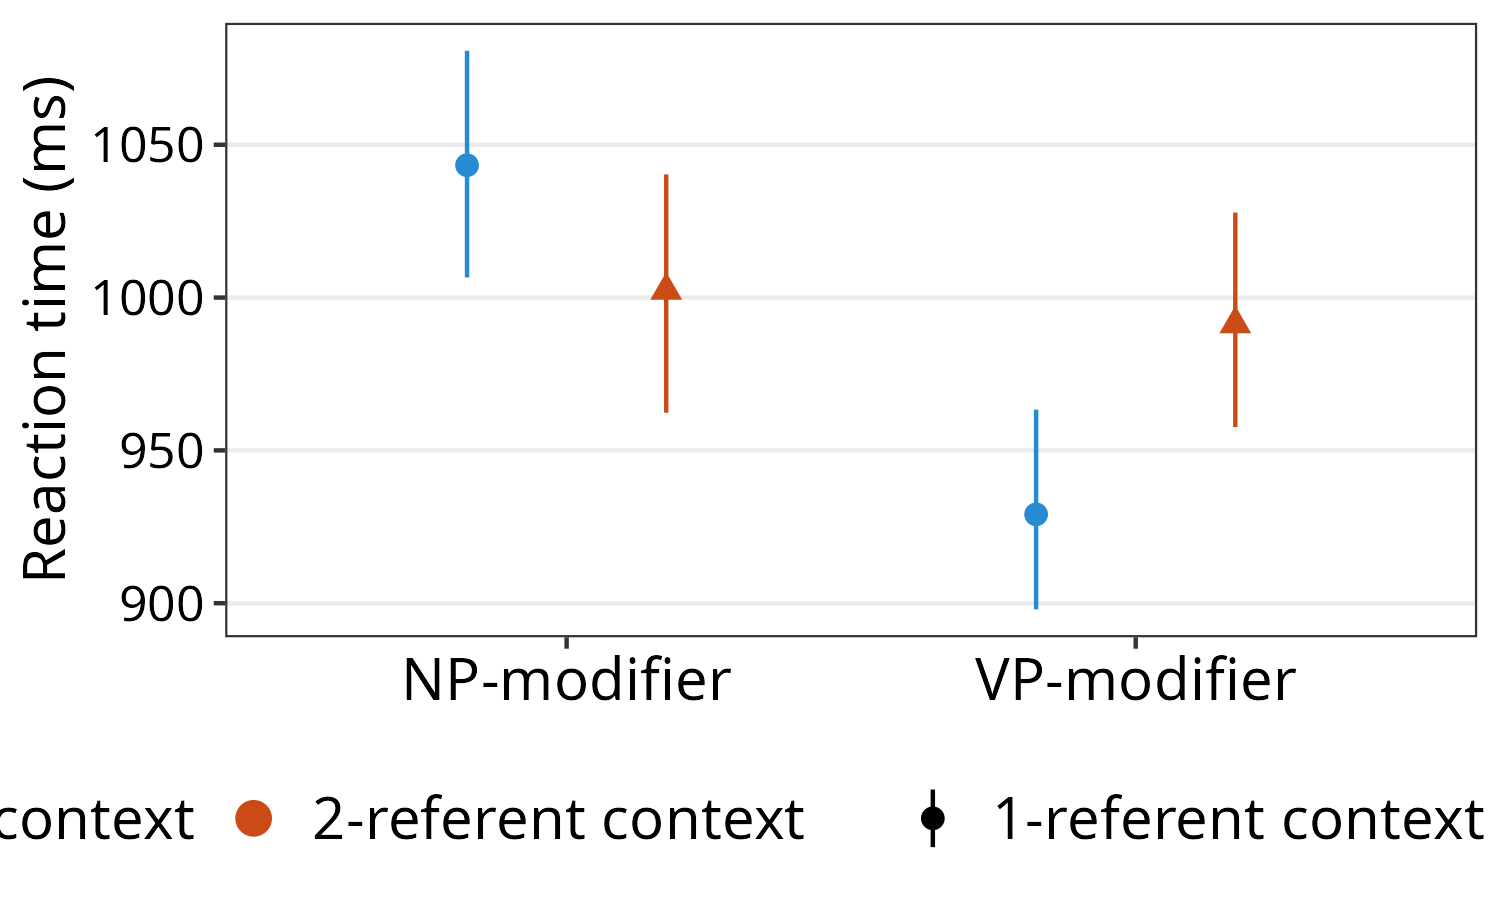
\includegraphics[width=\textwidth]{nrsa.png}} 
		\begin{small}
			CAPTION HERE
			
		\end{small}
		
	\end{minipage}
	~~~
	\begin{minipage}{.5\textwidth}	
		\begin{tabular}{l}
			TODO results table here\\
		\end{tabular}
	\end{minipage}

\begin{minipage}{\textwidth}
	\begin{small} \textbf{References:}
		
		TODO update
Leung, Hawkins, Yurovsky. Cogsci, 2020. $\bullet$ Glucksberg, Krauss, Weisberg. J of Expt Child Psychology, 1966. $\bullet$ Clark \& Wilkes-Gibbs. Cognition, 1986. $\bullet$ Hawkins, Frank, Goodman. Cognitive Science, 2020. $\bullet$ Reimers \& Gurevych. arXiv 2019.
\end{small}
\end{minipage}


\end{document}